\documentclass[t]{beamer}
\usecolortheme[RGB={0,114,197}]{structure} 
\usetheme{Ilmenau} 
\usepackage{tikz}
\usepackage{multicol}

\title{Software-Ontwerp}
\subtitle{Iteratie 1}
\author{Reniers V. - Devlieghere J. - Castel D. - Pante S.}
\institute{KU Leuven}

\begin{document}

\frame{\titlepage} 
\begin{frame}{Inhoud}
\begin{multicols}{2}
\tableofcontents
\end{multicols}
\end{frame}



\section{Inleiding} 
\begin{frame}{Inleiding} 
Thema's die aan bod komen:
\begin{itemize}
	\item High-Level bespreking van het ontwerp.
	\item Onderdelen in detail bekeken.
	\item GRASP en design patterns.
	\item Uitbreidbaarheid van het ontwerp.
	\item Test cases.
\end{itemize}
\end{frame}

\subsection{Rolverdeling}
\begin{frame}{Componenten}
\begin{multicols}{2}
\tableofcontents[currentsection]
\end{multicols}
\end{frame}

\begin{frame}{Rolverdeling}
Iteratie 1:
\begin{itemize}
	\item Lead Designer: Stefan Pante
	\item Lead Tester: Dieter Castel
\end{itemize}

Iteratie 2:
\begin{itemize}
	\item Lead Designer: Dieter Castel 
	\item Lead Tester: Vincent Reniers
\end{itemize}
\end{frame}

\section{Het ontwerp}
\subsection{Basisstructuur}
\begin{frame}{Componenten}
\begin{multicols}{2}
\tableofcontents[currentsection]
\end{multicols}
\end{frame}

\begin{frame}{Basistructuur}
Packages:
\begin{itemize}
	\item Game
	\item Square
	\item Handlers
	\item Items
	\item Player
	\item GUI
\end{itemize}
Test-cases voor elke package.
\end{frame}


\subsection{UML}
\begin{frame}{Componenten}
\begin{multicols}{2}
\tableofcontents[currentsection]
\end{multicols}
\end{frame}

\begin{frame}[plain]
\begin{center}
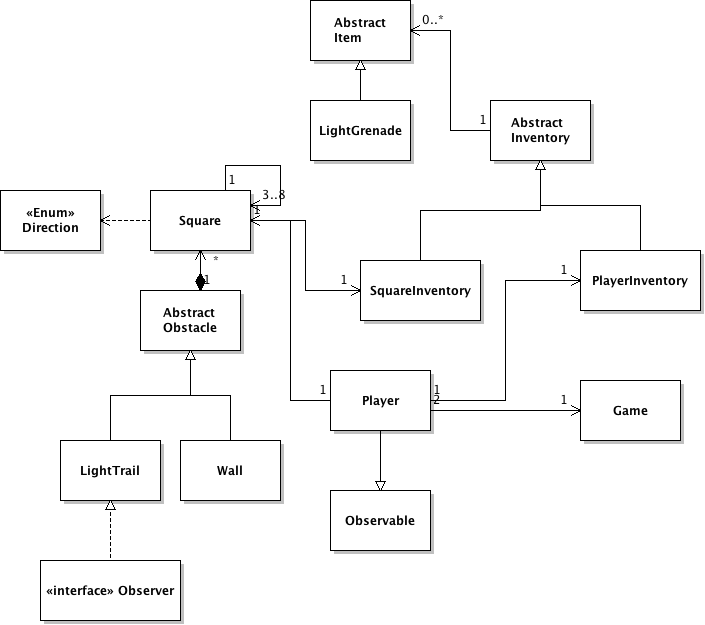
\includegraphics[width= 0.9\linewidth]{../uml/SimpleOverview.png}
\end{center}
\end{frame}

\section{Componenten}
\subsection{Obstacles}
\begin{frame}{Componenten}
\begin{multicols}{2}
\tableofcontents[currentsection]
\end{multicols}
\end{frame}

\begin{frame}[plain]{Square en obstacle}
\begin{center}
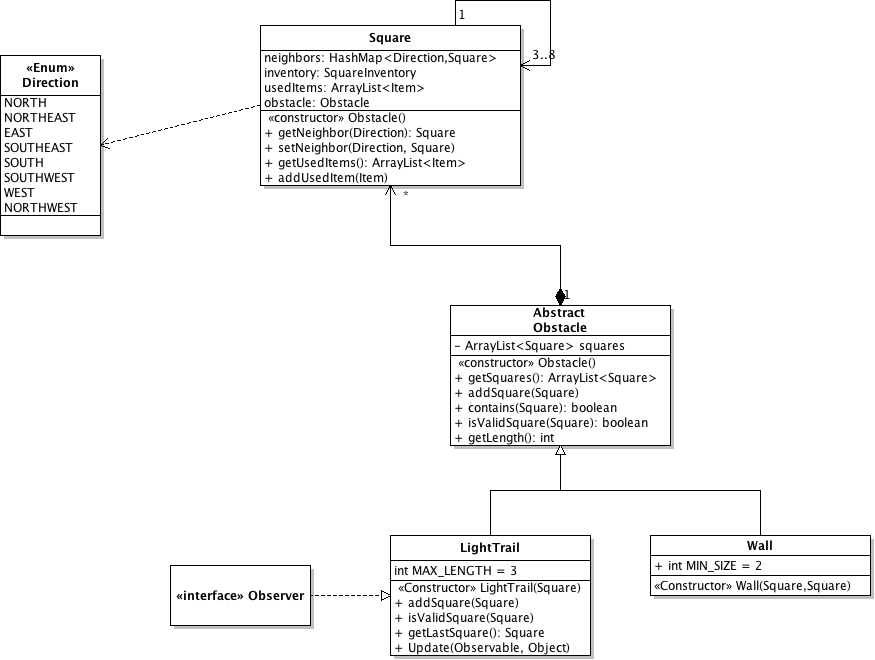
\includegraphics[width= 0.9\linewidth]{../uml/classdiagramObstaclesSquare.png}
\end{center}
\end{frame}

\subsection{Inventories}
\begin{frame}{Inventories}
\begin{multicols}{2}
\tableofcontents[currentsection]
\end{multicols}
\end{frame}

\begin{frame}[plain]{Items in Inventory}
\begin{center}
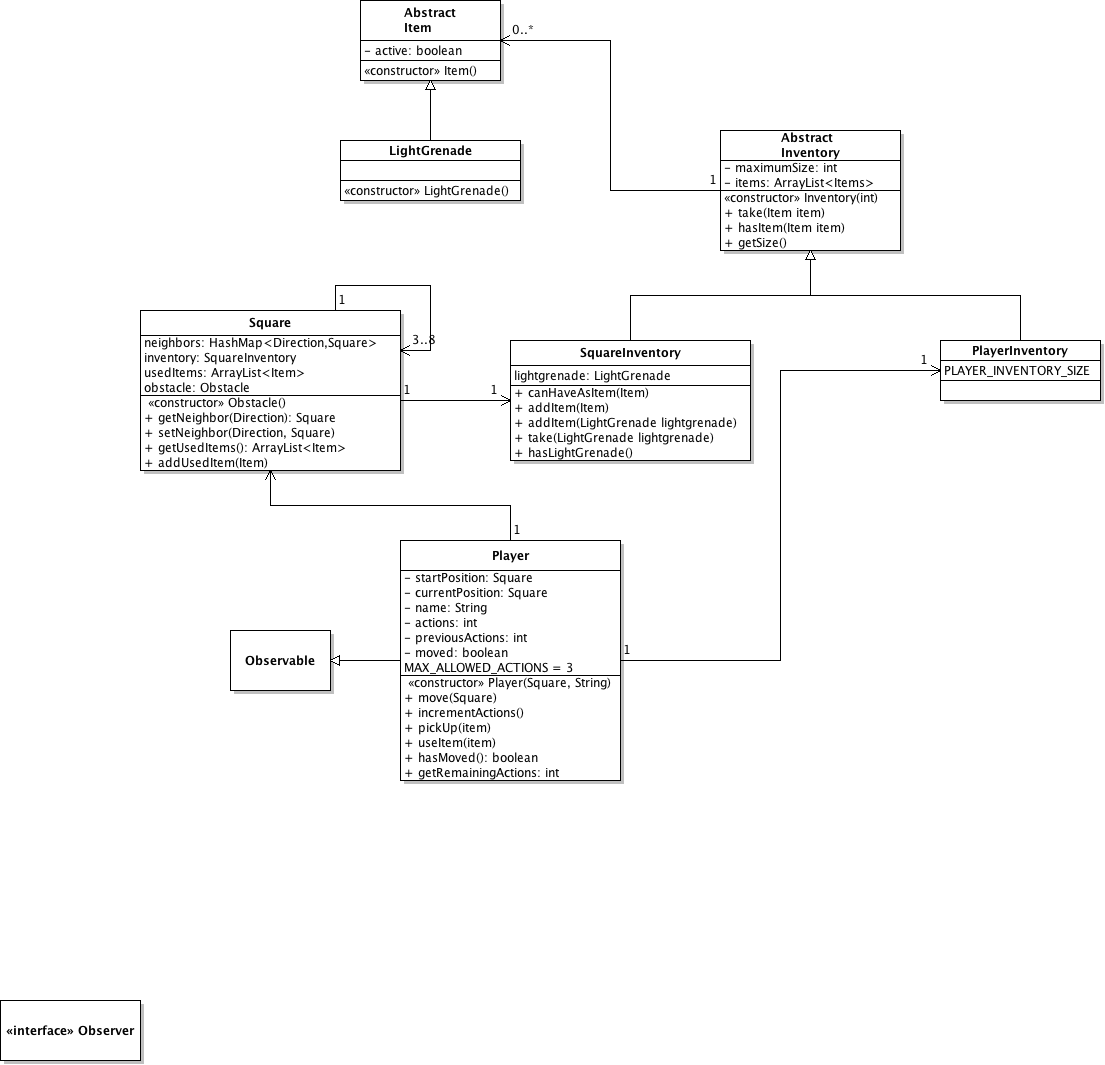
\includegraphics[width= 0.9\linewidth]{../uml/classdiagramInventory.png}
\end{center}
\end{frame}

\subsection{Grid constructie}
\begin{frame}{Inventories}
\begin{multicols}{2}
\tableofcontents[currentsection]
\end{multicols}
\end{frame}

\begin{frame}{Constructie van het Grid}
\begin{itemize}
	\item Klasse die een random grid genereert.
	\item Dit grid voldoet aan de verschillende constraints.
\end{itemize}

\begin{figure}
\begin{center}
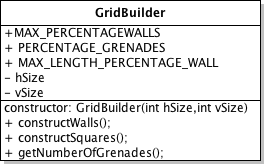
\includegraphics[scale=0.5]{../uml/gridBuilder.png}
\end{center}
\end{figure}

\end{frame}

\section{Interactie}
\begin{frame}{Interactie}
\begin{multicols}{2}
\tableofcontents[currentsection]
\end{multicols}
\end{frame}

\begin{frame}{Onderlinge interactie}
Sequentie diagrammen van de use cases:
\begin{itemize}
	\item PickUp
	\item moveTo
	\item endTurn
	\item useItem
\end{itemize}
\end{frame}

% Item pick up
\subsection{Pick up}
\begin{frame}{Interactie}
\begin{multicols}{2}
\tableofcontents[currentsection]
\end{multicols}
\end{frame}

\begin{frame}[plain]
\begin{center}
\includegraphics[width= 0.90\linewidth]{../uml/pickup_SD.png}
\end{center}
\end{frame}

% Move to
\subsection{Move to}
\begin{frame}{Interactie}
\begin{multicols}{2}
\tableofcontents[currentsection]
\end{multicols}
\end{frame}

\begin{frame}[plain]
\begin{center}
\includegraphics[width= 1\linewidth]{../uml/move_SD.png}
\end{center}
\end{frame}

% End turn
\subsection{End Turn}
\begin{frame}{Interactie}
\begin{multicols}{2}
\tableofcontents[currentsection]
\end{multicols}
\end{frame}

\begin{frame}[plain]
\begin{center}
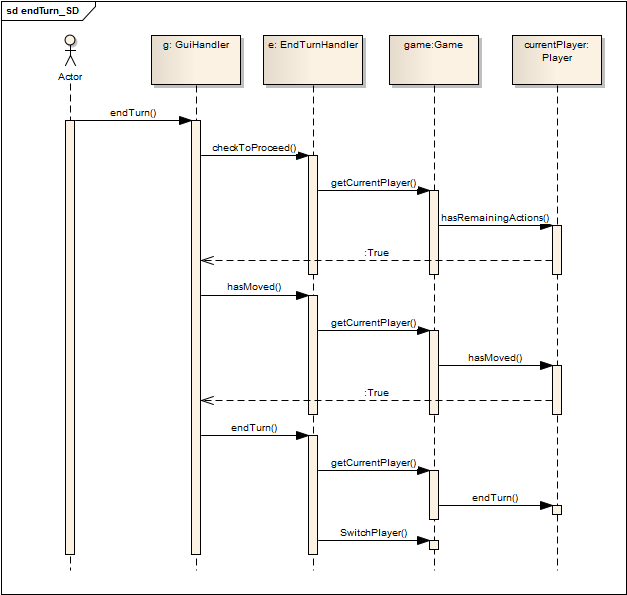
\includegraphics[width= 0.90\linewidth]{../uml/endTurn_SD.png}
\end{center}
\end{frame}

% Use Item
\subsection{Use item}
\begin{frame}{Interactie}
\begin{multicols}{2}
\tableofcontents[currentsection]
\end{multicols}
\end{frame}

\begin{frame}[plain]{Use Item}
\begin{center}
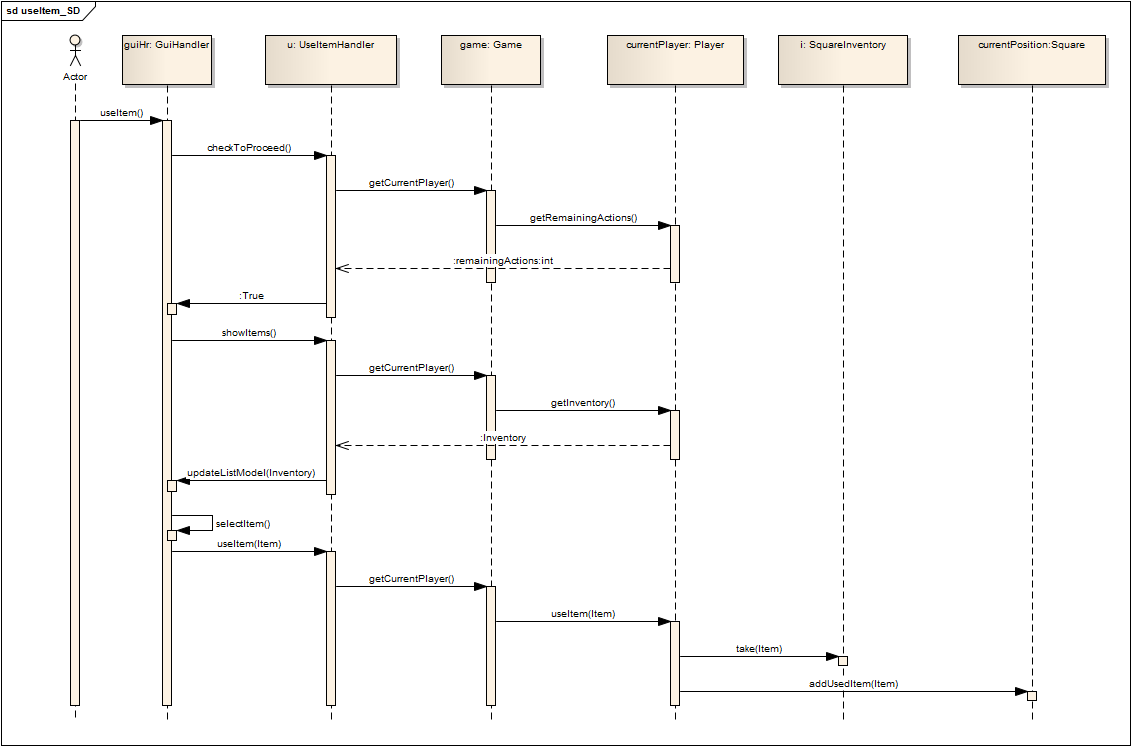
\includegraphics[width= 1\linewidth]{../uml/useItem_SD.png}
\end{center}
\end{frame}

\section{Test cases}
\subsection{JUnit}
\begin{frame}{Test cases}
\begin{multicols}{2}
\tableofcontents[currentsection]
\end{multicols}
\end{frame}

\begin{frame}{JUnit test per klasse}
\begin{itemize}
	\item Test-Driven Development
	\begin{itemize}
		\item	Test klassen per klasse.
		\item	Methodes op voorhand uitwerking in Tests.
		\item	Gaandeweg extra tests bij nieuwe functionaliteit.
	\end{itemize}
\end{itemize}
\end{frame}

\subsection{Eclemma}
\begin{frame}{Test cases}
\begin{multicols}{2}
\tableofcontents[currentsection]
\end{multicols}
\end{frame}

\begin{frame}[plain]{Eclemma}
Voldoende tests en coverage in onderste lagen van het model.
\begin{center}
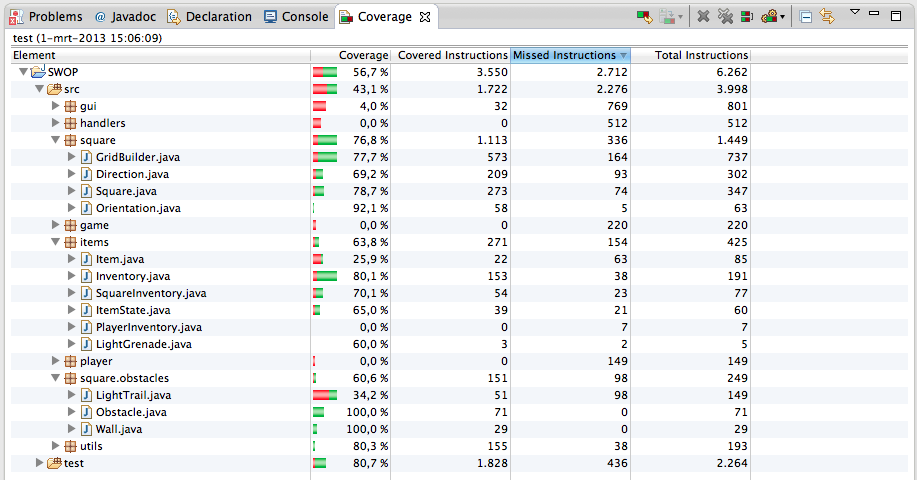
\includegraphics[width= 1\linewidth]{images/coverage.png}
\end{center}
\end{frame}


\section{Uitbreidbaarheid}
\subsection{Polymorfisme}
\begin{frame}{Uitbreidbaarheid}
\begin{multicols}{2}
\tableofcontents[currentsection]
\end{multicols}
\end{frame}

\begin{frame}{Polymorfisme}
Overerving vindt plaats via:
\begin{itemize}
	\item Obstacle \textit{(voor Wall, LightTrail)}
	\item Inventory \textit{(voor PlayerInventory, SquareInventory)}
	\item Item	\textit{(voor LightGrenade)}
\end{itemize}
\end{frame}

\begin{frame}[plain]{Polymorfisme}
\begin{center}
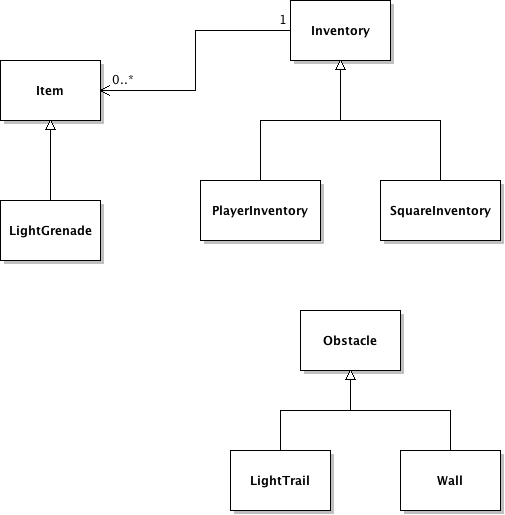
\includegraphics[width= 0.6\linewidth]{../uml/polymorphism.png}
\end{center}
\end{frame}

\subsection{Modulair design}
\begin{frame}{Uitbreidbaarheid}
\begin{multicols}{2}
\tableofcontents[currentsection]
\end{multicols}
\end{frame}

\begin{frame}[plain]{Modulair design}
\begin{center}
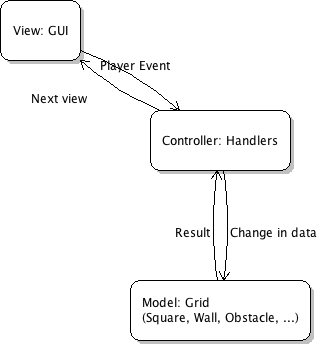
\includegraphics[width= 0.5\linewidth]{../uml/MVC.png}
\end{center}
\end{frame}

\begin{frame}{Besluit}
\vspace{0.8in}
\begin{center}
Bedankt voor uw aandacht.
\end{center}
\end{frame}

\end{document}
